% =====================================================================
% Figura 5 — Rede temática do corpus bibliográfico.
%
% Substitui grafico_4_rede_tematica_sem_margem.png. A versão anterior
% deixava um quadrante inteiro vazio e distribuía os nós sem relação com
% a distância conceitual que o texto descreve. Aqui o núcleo técnico
% ocupa o centro, o ramo de execução embarcada desce à direita e o ramo
% agrícola, descrito no texto como periférico, fica à esquerda.
%
% REQUER no preâmbulo (já presentes em artigo.tex):
%   \usepackage{tikz}
%   \usetikzlibrary{positioning, arrows.meta}
% =====================================================================

\begin{figure}[H]
    \centering
    \caption{Rede temática dos conceitos recorrentes no \textit{corpus} bibliográfico}
    \label{fig:rede_tematica}

    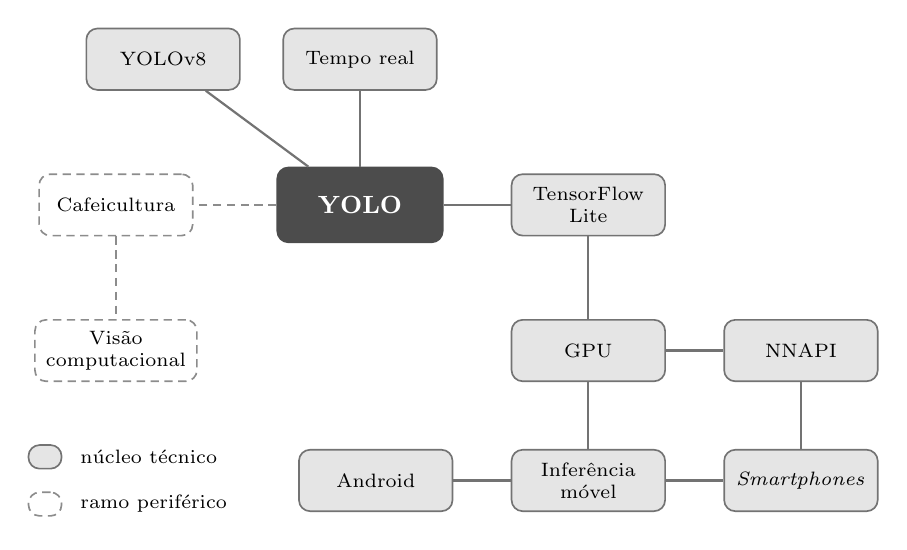
\begin{tikzpicture}[
        every node/.style={font=\scriptsize},
        no/.style={
            rectangle, rounded corners=4pt, draw, line width=0.6pt,
            align=center, inner sep=4pt, minimum height=0.78cm,
            minimum width=1.95cm
        },
        nucleo/.style={no, draw=black!70, fill=black!70, text=white,
                       font=\small\bfseries, minimum width=2.1cm,
                       minimum height=0.95cm},
        tecnico/.style={no, draw=black!55, fill=black!10},
        periferico/.style={no, draw=black!45, fill=white,
                           densely dashed},
        lig/.style={draw=black!55, line width=0.8pt},
        ligp/.style={draw=black!45, line width=0.8pt, densely dashed}
    ]

    % ------------------------------------------------- núcleo
    \node[nucleo] (yolo) at (0,0) {YOLO};

    % ------------------------------------------------- ramo de detecção
    \node[tecnico] (v8)    at (-2.5, 1.85) {YOLOv8};
    \node[tecnico] (tempo) at ( 0.0, 1.85) {Tempo real};
    \node[tecnico] (tfl)   at ( 2.9, 0.00) {TensorFlow\\Lite};

    % --------------------------------------- ramo de execução embarcada
    \node[tecnico] (gpu)   at ( 2.9,-1.85) {\ac{GPU}};
    \node[tecnico] (nnapi) at ( 5.6,-1.85) {\ac{NNAPI}};
    \node[tecnico] (infm)  at ( 2.9,-3.50) {Inferência\\móvel};
    \node[tecnico] (andr)  at ( 0.2,-3.50) {Android};
    \node[tecnico] (smart) at ( 5.6,-3.50) {\textit{Smartphones}};

    % ------------------------------------------------- ramo agrícola
    \node[periferico] (cafe) at (-3.1, 0.00) {Cafeicultura};
    \node[periferico] (visao) at (-3.1,-1.85) {Visão\\computacional};

    % ------------------------------------------------- arestas
    \draw[lig] (yolo) -- (v8);
    \draw[lig] (yolo) -- (tempo);
    \draw[lig] (yolo) -- (tfl);
    \draw[lig] (tfl)  -- (gpu);
    \draw[lig] (gpu)  -- (nnapi);
    \draw[lig] (gpu)  -- (infm);
    \draw[lig] (infm) -- (andr);
    \draw[lig] (infm) -- (smart);
    \draw[lig] (nnapi) -- (smart);
    \draw[ligp] (yolo) -- (cafe);
    \draw[ligp] (cafe) -- (visao);

    % ------------------------------------------------- legenda interna
    \node[tecnico, minimum width=0.42cm, minimum height=0.30cm,
          inner sep=0pt] (lg1) at (-4.0,-3.20) {};
    \node[anchor=west, font=\scriptsize] at ([xshift=3pt]lg1.east)
        {núcleo técnico};
    \node[periferico, minimum width=0.42cm, minimum height=0.30cm,
          inner sep=0pt] (lg2) at (-4.0,-3.80) {};
    \node[anchor=west, font=\scriptsize] at ([xshift=3pt]lg2.east)
        {ramo periférico};

    \end{tikzpicture}

    \legend{Elaborada pela autora (2026).}
\end{figure}
